\documentclass[a4paper,11pt]{article}
\usepackage{amsmath}
\usepackage{graphicx}
\usepackage{hyperref}
\usepackage{geometry}
\usepackage{listings}
\geometry{margin=1in}
\hypersetup{
    colorlinks=true,
    linkcolor=blue,
    urlcolor=blue
}
\usepackage{float}

\title{REPORT: Mixture of Experts (MoE) Model for Image Processing}
\author{Carlos Garcia}
\date{\today}

\begin{document}

\maketitle

\section{Introduction}
Mixture of Experts (MoE) models have gained significant attention due to their ability to combine multiple specialized models (``experts") for improving the performance of deep learning architectures. While MoE models are traditionally applied in natural language processing (NLP) \cite{shazeer2017outrageously}, this report explores their adaptation to image processing tasks. Specifically, we implement and evaluate a transformer-based MoE model for image classification.

\section{Mixture of Experts (MoE) Overview}
MoE is a concept where different ``experts" are selected dynamically based on the input data. In the MoE architecture, each input is routed to a subset of these experts, typically using a gating mechanism, ensuring that only the most relevant experts are utilized at any given time. This approach not only reduces computational cost but also increases flexibility and specialization in the model \cite{huggingfaceMixtureExperts}.

For this project, the transformer architecture \cite{vaswani2017attention} is adapted, where the feed-forward layers in the transformer blocks are replaced with expert layers. These expert layers consist of multiple expert networks, with a gating mechanism determining which experts are activated for a given input. The MoE mechanism for image processing introduces unique challenges compared to its application in NLP, particularly in handling the two-dimensional structure of images.

\section{Model Implementation}
The model is implemented in PyTorch \cite{pytorch}, leveraging the MoE design to replace feed-forward layers in a transformer encoder block with specialized expert layers. We use the MNIST dataset \cite{lecun1998mnist}, which is widely used for benchmarking image classification models.

The implementation consists of:
\begin{itemize}
    \item \textbf{Experts}: Each expert is a simple feed-forward network composed of two linear layers with a GELU activation function \cite{hendrycks2020gaussian}.
    \item \textbf{Gating Mechanism}: A learned linear layer is used to route input data to a selected subset of experts based on the top-k gating strategy.
    \item \textbf{Transformer Architecture}: A traditional transformer encoder is employed, where MoE layers are integrated. The transformer processes image patches extracted from the MNIST dataset. The model is trained using a standard cross-entropy loss function. The model architecture uses concepts from the Vision Transformer (ViT) \cite{dosovitskiy2020image}.
    \item \textbf{Training Pipeline}: The model is trained using the Adam optimizer \cite{kingma2014adam} and the GELU activation function \cite{hendrycks2016gaussian}. The training pipeline is tracked using MLFlow \cite{mlflow} and DAGsHub \cite{dagshub}.
    \item \textbf{Hyperparameter Tuning}: Key hyperparameters such as the number of experts, top-k selection, patch size, and expert placement are tuned to optimize the model's performance (See the 'MoELayer' class in the repository, file 'nb\_moe.ipynb').
\end{itemize}

% \begin{lstlisting}[language=Python]
% class MoELayer(nn.Module):
%     def __init__(self, num_experts, d_model, d_ff, k=2):
%         super().__init__()
%         self.num_experts = num_experts
%         self.k = k
%         self.gate = nn.Linear(d_model, num_experts)
%         self.experts = nn.ModuleList([Expert(d_model, d_ff) for _ in range(num_experts)])

%     def forward(self, x):
%         batch_size, seq_len, d_model = x.shape
%         gate_outputs = self.gate(x)
%         top_k_gates, top_k_indices = torch.topk(gate_outputs, self.k, dim=-1)
%         top_k_gates = torch.softmax(top_k_gates, dim=-1)
%         expert_outputs = torch.zeros_like(x).unsqueeze(-2).repeat(1, 1, self.k, 1)
%         for i in range(self.k):
%             idx = top_k_indices[:, :, i]
%             expert_outputs[:, :, i, :] = torch.stack([self.experts[idx[b, s]](x[b, s]) for b in range(batch_size) for s in range(seq_len)]).view(batch_size, seq_len, -1)
%         output = torch.sum(top_k_gates.unsqueeze(-1) * expert_outputs, dim=2)
%         return output
% \end{lstlisting}

\section{Training and Experimentation}
The training is conducted on the MNIST dataset, with a transformer model configured to use MoE layers. Key hyperparameters such as the number of experts, patch size, and placement of experts were varied in the experiments. The training pipeline was tracked using MLFlow \cite{mlflow} and DAGsHub \cite{dagshub}. Since computational resources were limited, the training time was an important factor to consider for the experiments, which were splitted into five stages:

\begin{itemize}
    \item \textbf{Number of Experts and Top-k Selection}: 
    The values tested were combinations of the parameters $num\_experts = [2, 4, 8, 16, 32]$ and $topk = [2, 4, 8]$. A good balance between the accuracy and computational cost was found with $num\_experts = 4$ and $topk = 2$ (Figure \ref{fig:experts_topk}), which was used as the base configuration for the subsequent experiments.

    % ----------------
    
    \item \textbf{Patch Size}: The influence of patch size on the model's performance was systematically evaluated. While smaller patch sizes enable the model to capture finer details, they also significantly increase the computational costs, sometimes not even converging to a good solution. The patch sizes tested were $patch\_size  [4, 8, 16, 32]$. The best balance between accuracy and computational cost was found with a patch size of $16 \times 16$. See Figure \ref{fig:patch_size}.

    % ----------------

    \item \textbf{Number of Layers and Expert Placement}: First I did tests on the number of layers, the values tested were $n\_layers = [2, 3, 4, 5]$. I found that the best balance between accuracy and computational cost was with $n\_layers = 3$. Then I tested the placement of the experts in the transformer layers, the values tested were $expert\_placement = ['all', [0], [1], [2], [0, 2]]$. The best results were obtained when the experts were placed in the middle of the transformer layers ($expert\_placement = [[2]]$). See Figure \ref{fig:layers_placement}. In general, the model performed better when the experts were placed not too early or too late in the transformer layers, and not in all layers.

    % ----------------

    \item \textbf{Learning Rate}: The learning rate was tuned to find the optimal value for the model. The values tested were $learning\_rate = [0.01, 0.005, 0.001, 0.0005, 0.0001, 0.00005]$. The best results were obtained with a learning rate of $0.0001$. See Figure \ref{fig:learning_rate}.

    % ----------------

    \item \textbf{Long Run}: A long run with 50 epochs was conducted to observe the model's convergence and determine if it overfits the training data. The results are shown in Figure \ref{fig:long_run}.

    % ----------------

\end{itemize}


\section{Results}
The results of the experiments are summarized below:

\begin{itemize}
    \item \textbf{Base Configuration}: The base configuration of the MoE model achieved an accuracy of \textbf{XX\%} on the MNIST test dataset.
    \item \textbf{Optimal Hyperparameters}: The optimal hyperparameters for the MoE model were found to be:
    \begin{itemize}
        \item Number of Experts: 4
        \item Top-k Selection: 2
        \item Patch Size: $16 \times 16$
        \item Number of Layers: 3
        \item Expert Placement: Middle of the transformer layers
        \item Learning Rate: 0.0001
    \end{itemize}
    \item \textbf{Long Run Performance}: The model achieved a test accuracy of \textbf{XX\%} after \textbf{N} epochs in the long run experiment.
\end{itemize}

% Let's create a 'baselines' section to compare the MoE model with other models. 
% make two examples with CNN and Standard Transformers model to compare with our results. Use them as baseline.
\section{Baselines}
To evaluate the performance of the MoE model, we compare it with two baseline models: a Convolutional Neural Network (CNN) (See file 'nb\_baseline\_cnn.ipynb' in the repository) and a standard Transformer model (See file 'nb\_baseline\_transformer' in the repository). The CNN model consists of multiple convolutional layers followed by fully connected layers, while the standard Transformer model uses self-attention mechanisms to process the image patches.

Figure \ref{fig:baselines} shows that the MoE model (red) takes longer to converge compared to the CNN (brown), but it eventually matches its accuracy at around 99\%. The Transformer model (yellow), while improving early on, fluctuates significantly and underperforms compared to both the CNN and MoE models. 

MoE's strength lies in its scalability; it can handle larger datasets more efficiently by distributing the computational load across multiple experts, making it ideal for complex image processing tasks. As datasets grow, MoE models can provide better resource allocation and adaptivity, leading to improved performance with high-dimensional data.

\section{Conclusion}
The Mixture of Experts model demonstrates promising results for image classification tasks. By dynamically selecting experts, the model can balance computation and performance, making it an efficient choice for resource-constrained scenarios. Future work could explore applying this model to larger and more complex datasets, as well as optimizing the training pipeline for faster convergence and to include more hyperparameters in the experiments such as batch size, dropout, and weight decay. Additionally, we could include a load balancing loss term to encourage more even use of experts and apply further visualization techniques to analyze the behavior of different experts for different types of inputs.


% --------------------------------------------

\section{Resources}

\begin{itemize}
    \item \textbf{Code Repository}: \url{www.github.com/your-repo}
    \item \textbf{Main Model and training notebook}: \url{www.github.com/your-repo/nb_moe.ipynb}
    \item \textbf{DAGsHub Project}: \url{www.dagshub.com/your-username/your-project}
    \item \textbf{MNIST Dataset}: \url{www.mnist.org}
\end{itemize}

% --------------------------------------------

\section{Inspiration}

This are some of the materials that inspired the approach taken in this project:

\begin{itemize}

    \item \textbf{Mixture of Experts Explained}: \url{https://huggingface.co/blog/moe}
    \item \textbf{makeMoE_from_Scratch}: \url{https://colab.research.google.com/github/AviSoori1x/makeMoE/blob/main/makeMoE_from_Scratch.ipynb?authuser=0#scrollTo=90vgVgmDkRJQ}
    \item \textbf{makemore}: \url{https://github.com/karpathy/makemore/tree/master}
    \item \textbf{Fine-Tune ViT for Image Classification with Transformers }: \url{https://huggingface.co/blog/fine-tune-vit}
    \item \textbf{Vision Transformer (ViT)}: \url{https://huggingface.co/docs/transformers/en/model_doc/vit}
    
\end{itemize}

% --------------------------------------------

\section{Appendix}
\begin{figure}[H]
    \centering
    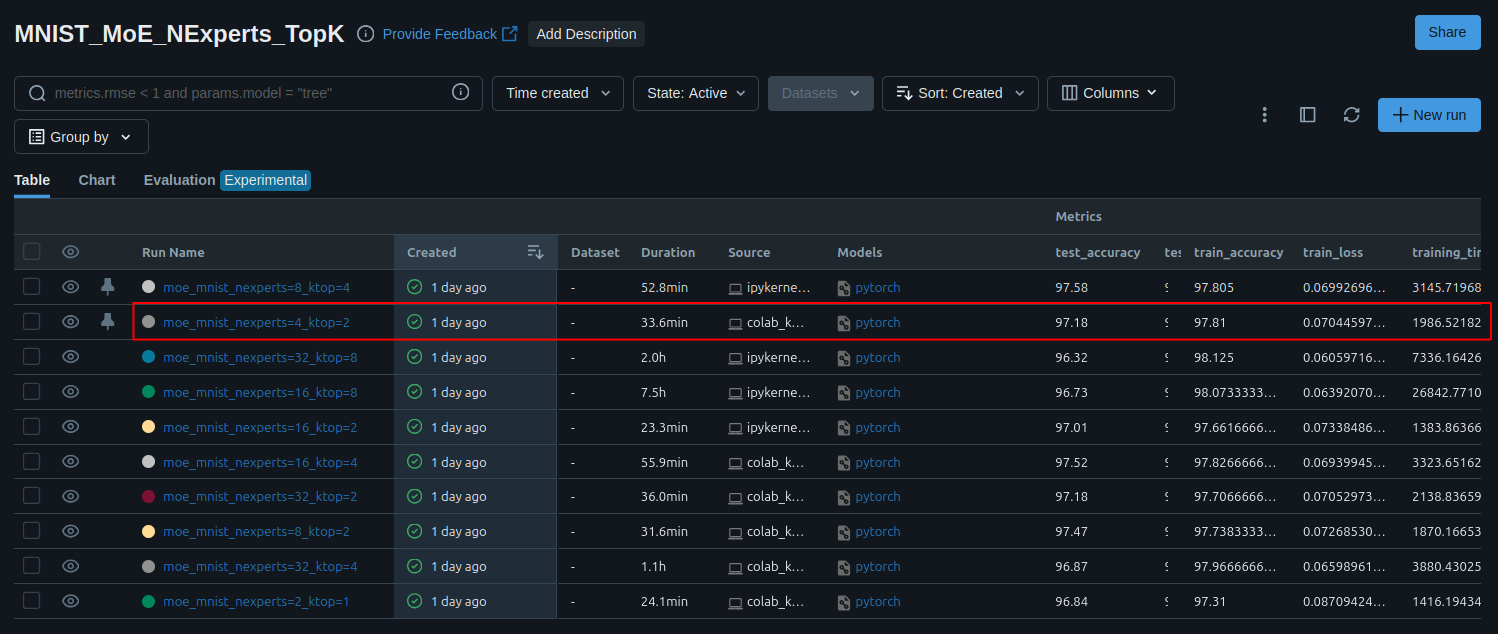
\includegraphics[width=0.6\textwidth]{images/experts_topk.png}
    \caption{Accuracy vs. Number of Experts and Top-k Selection}
\end{figure}

\begin{figure}[H]
    \centering
    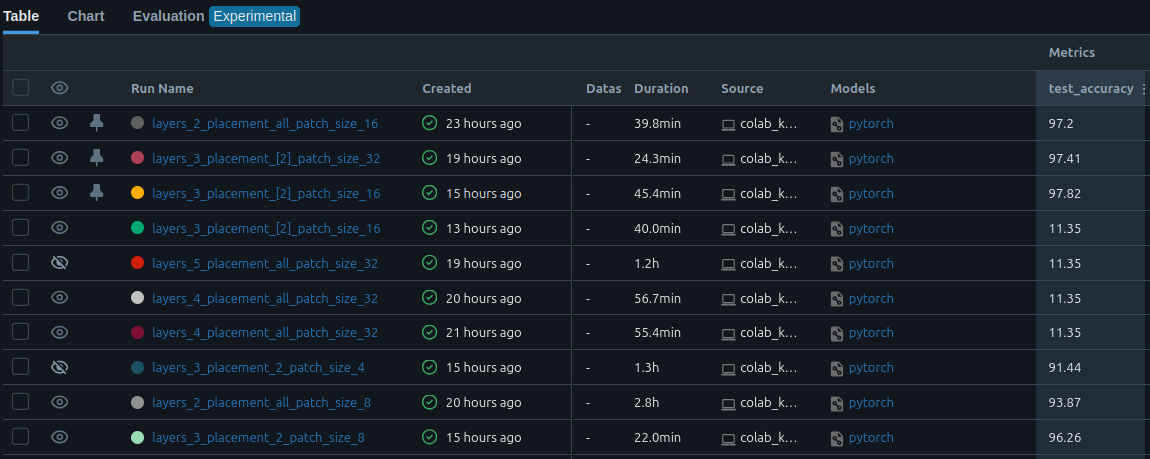
\includegraphics[width=0.6\textwidth]{images/patch_size.png}
    \caption{Accuracy vs. Patch Size}
\end{figure}

\begin{figure}[H]
    \centering
    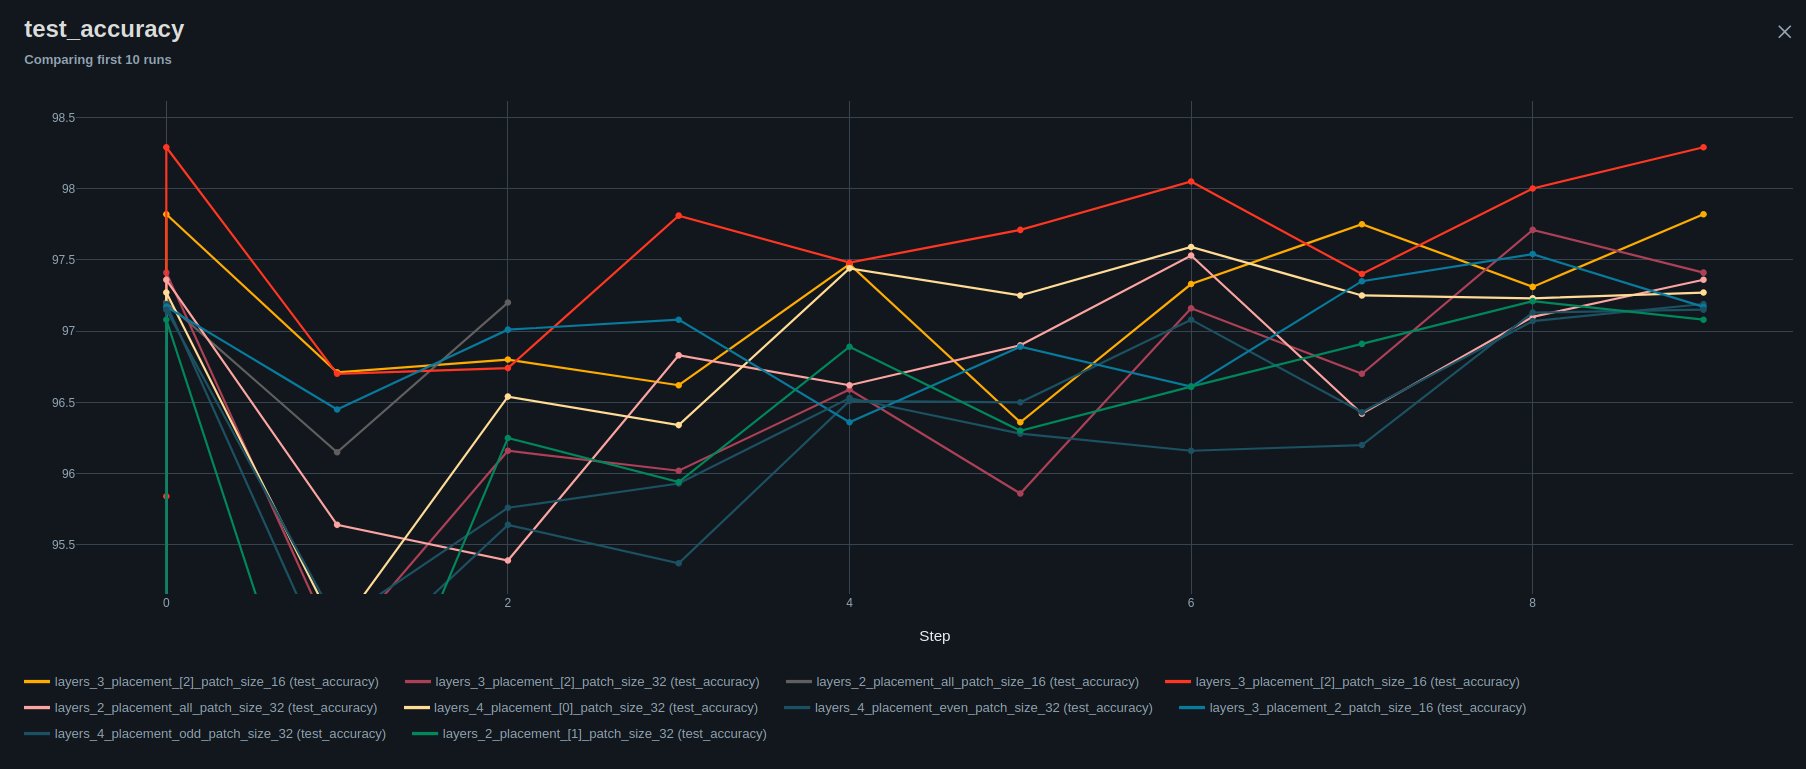
\includegraphics[width=0.6\textwidth]{images/layers_placement.png}
    \caption{Accuracy vs. Number of Layers and Expert Placement}
\end{figure}

\begin{figure}[H]
    \centering
    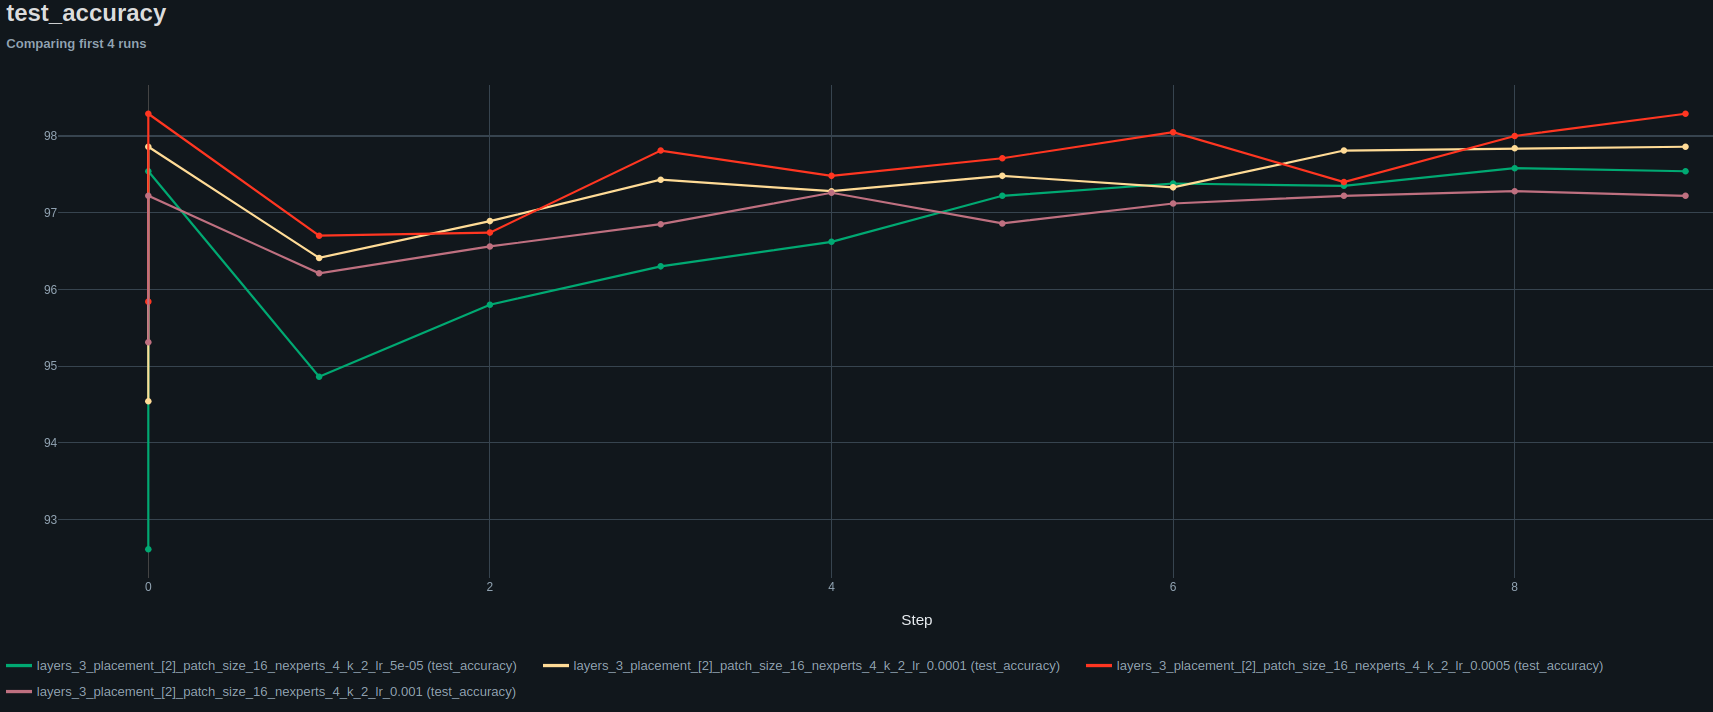
\includegraphics[width=0.6\textwidth]{images/learning_rate.png}
    \caption{Accuracy vs. Learning Rate}
\end{figure}

\begin{figure}[H]
    \centering
    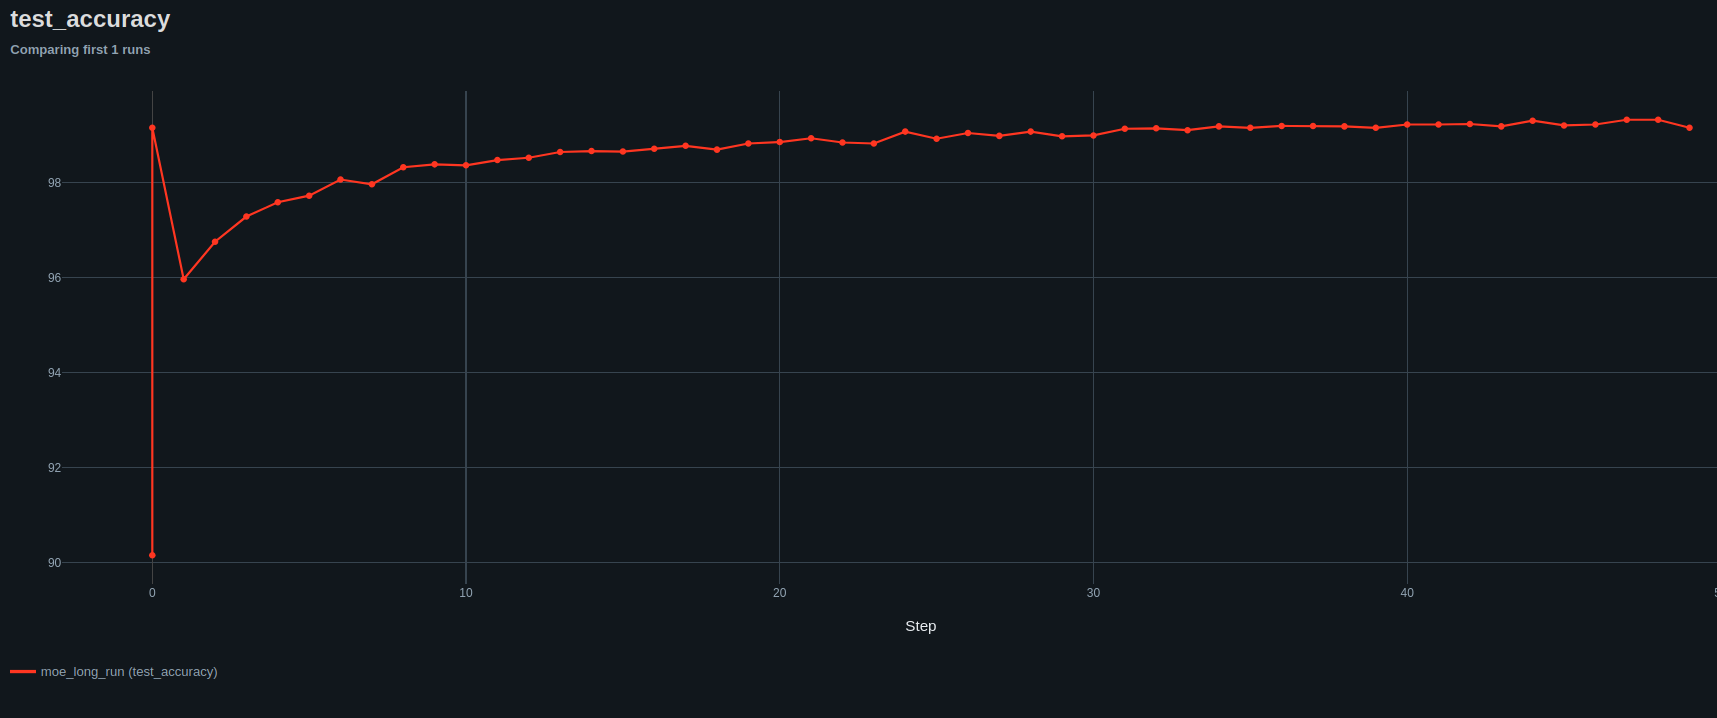
\includegraphics[width=0.6\textwidth]{images/long_run.png}
    \caption{Accuracy vs. Epochs (Long Run)}
\end{figure}

\begin{figure}[H]
    \centering
    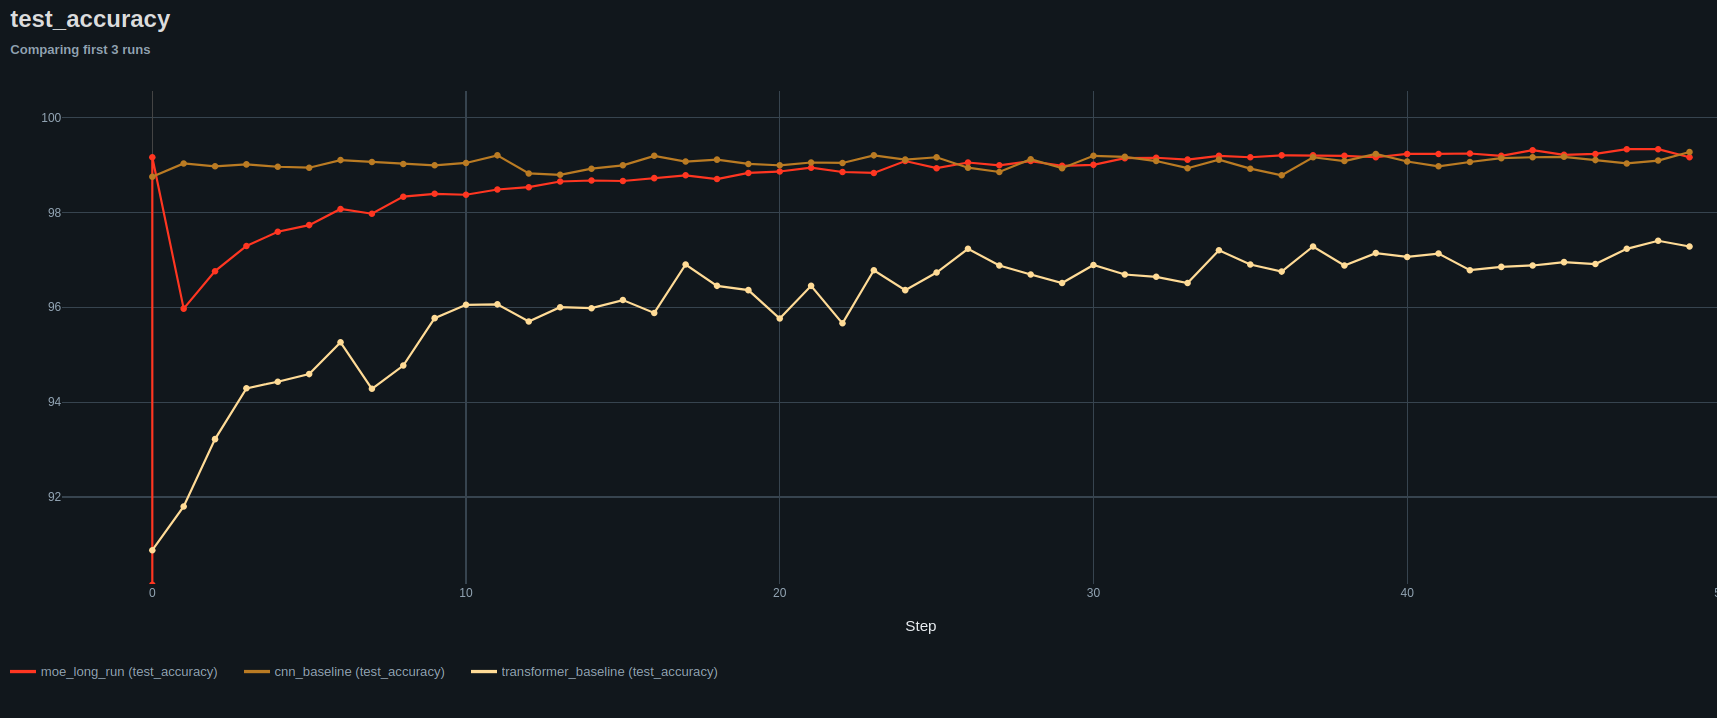
\includegraphics[width=0.6\textwidth]{images/baselines.png}
    \caption{Comparison of MoE Model with CNN and Standard Transformer}
\end{figure}

% --------------------------------------------

\section{References}

\renewcommand{\section}[2]{}%
%\renewcommand{\chapter}[2]{}% for other classes

\bibliographystyle{plain}
\bibliography{references}

\end{document}